\section{Discussion of Results}
\label{sec:discussionofresults}

\subsection{Influence of some parameters in our model}
\subsubsection{Influence of \texttt{noize}}
\label{sec:influencenoize}
As figure \ref{influencenoize} shows, the noize could have quite an influence on the results of the simulation. In our network we have in total 1200 nodes. All the simulations in figure \ref{influencenoize} have the same \texttt{maxUpdate}=0.02. This means that in every time step 24 agents get updated. If the noize is now for example 0.01 only 0.24 agents choose randomly their state. In the case of a noize of 0.1 get 2.4 agents every time step a randomly after a uniform distribution chosen mind state. After this "noize update" the concerned agents are removed from the sequential update list so that they could not be updated twice.\\
As figure \ref{influencenoize} now shows and explained above a noize of 0.01 does not really change the results of the simulation as it has nearly no influence. But as the series of five plots on the right in figure \ref{influencenoize} shows a noize of 10 $\%$ does have quite a big influence on the results of the simulation. Before this big noize the riots where not really starting in the networks now they spread quickly.\\
Compared to reality we think that the noize tends to be close to 0. Who is just completly random changing his mind? It could be that some people change their mind independently from their neighbors and these should be covered by the noize. We think that a noize in reality should be something between 0 and 0.06.

\begin{figure}
\centering
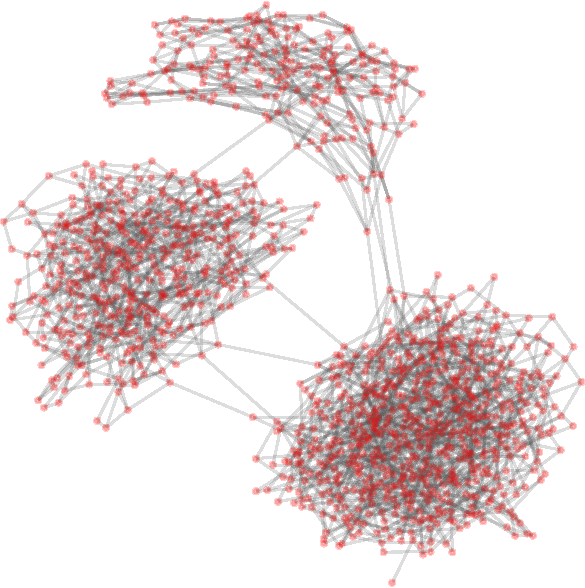
\includegraphics[width=0.25\textwidth]{batchRun__kHalf=2-2-2_maxUpdate=0.02_noize=0_nbrDepth=1/network0-crop.pdf}
\hfill
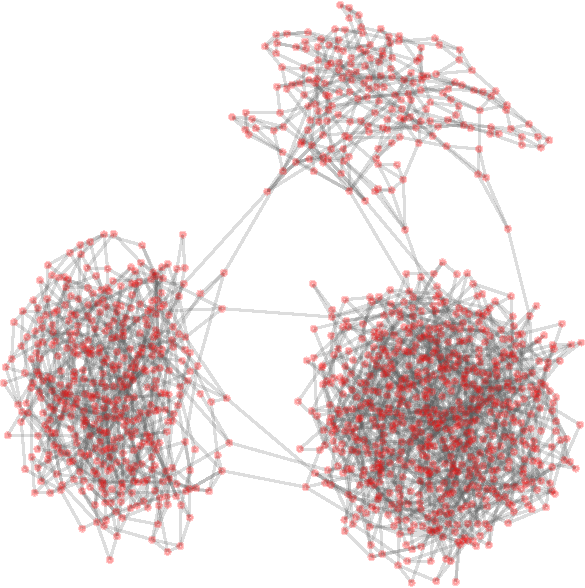
\includegraphics[width=0.25\textwidth]{batchRun__kHalf=2-2-2_maxUpdate=0.02_noize=0.01_nbrDepth=1/network0-crop.pdf}
\hfill
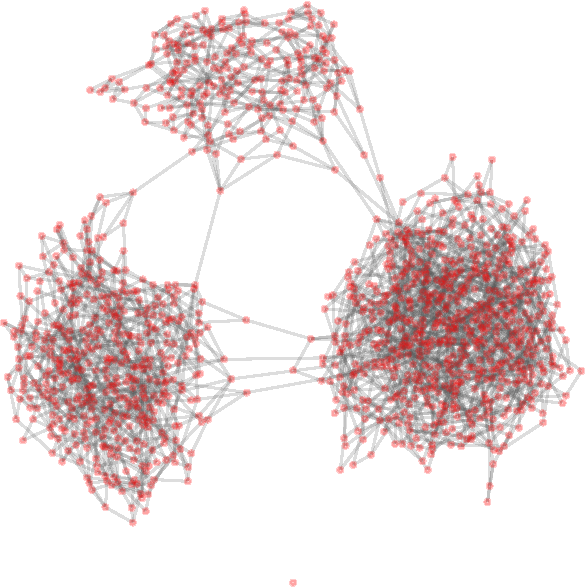
\includegraphics[width=0.25\textwidth]{batchRun__kHalf=2-2-2_maxUpdate=0.02_noize=0.1_nbrDepth=1/network0-crop.pdf}

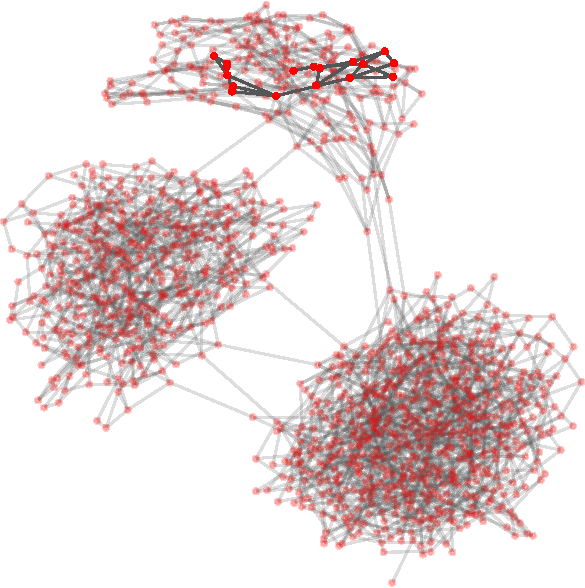
\includegraphics[width=0.25\textwidth]{batchRun__kHalf=2-2-2_maxUpdate=0.02_noize=0_nbrDepth=1/network250-crop.pdf}
\hfill
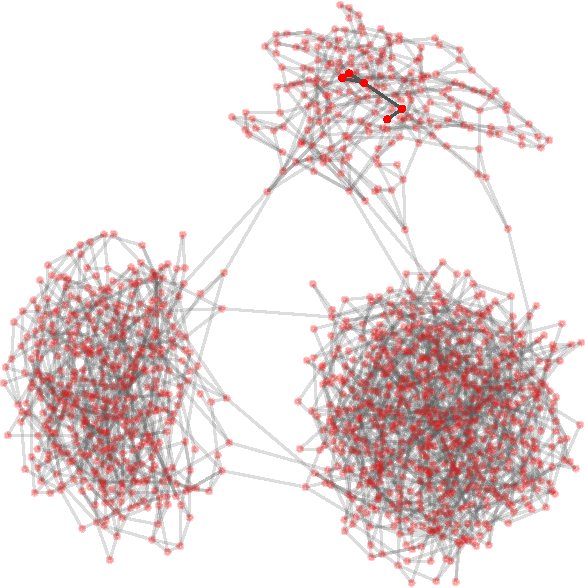
\includegraphics[width=0.25\textwidth]{batchRun__kHalf=2-2-2_maxUpdate=0.02_noize=0.01_nbrDepth=1/network250-crop.pdf}
\hfill
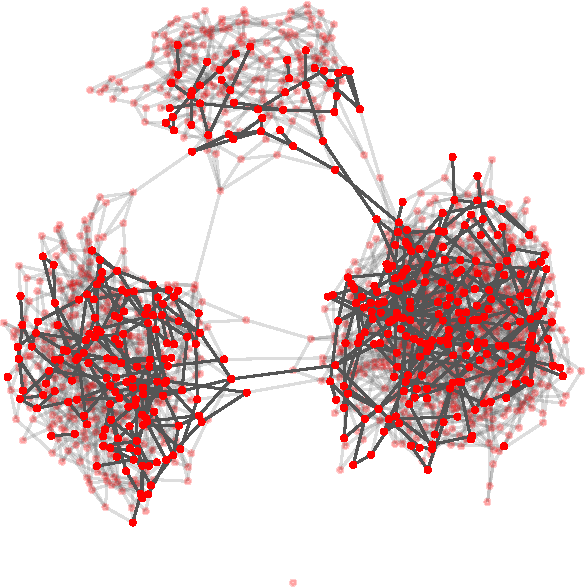
\includegraphics[width=0.25\textwidth]{batchRun__kHalf=2-2-2_maxUpdate=0.02_noize=0.1_nbrDepth=1/network250-crop.pdf}

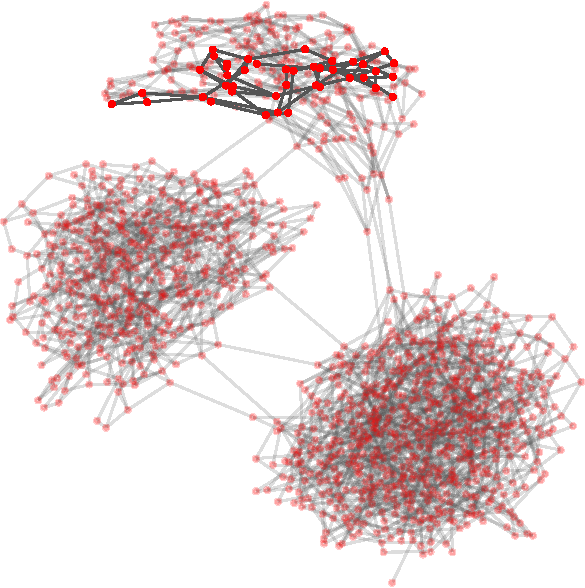
\includegraphics[width=0.25\textwidth]{batchRun__kHalf=2-2-2_maxUpdate=0.02_noize=0_nbrDepth=1/network500-crop.pdf}
\hfill
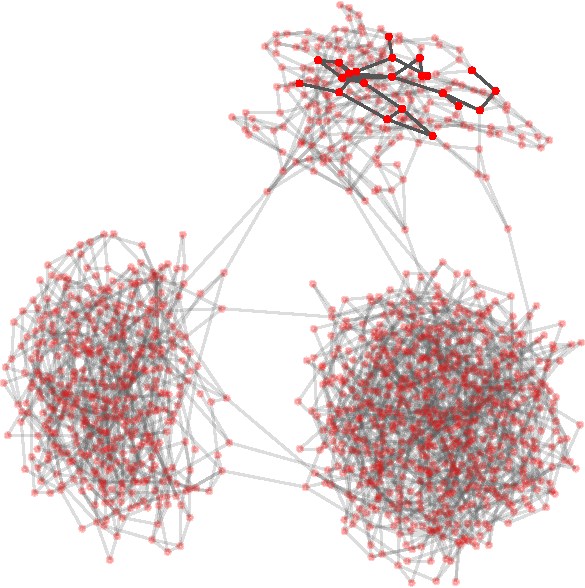
\includegraphics[width=0.25\textwidth]{batchRun__kHalf=2-2-2_maxUpdate=0.02_noize=0.01_nbrDepth=1/network500-crop.pdf}
\hfill
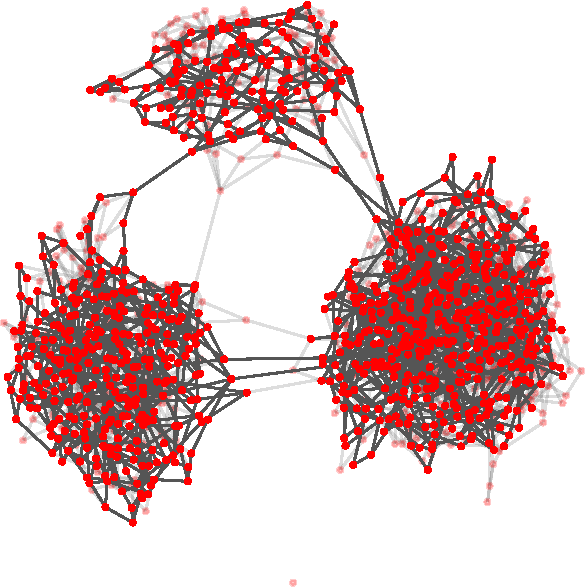
\includegraphics[width=0.25\textwidth]{batchRun__kHalf=2-2-2_maxUpdate=0.02_noize=0.1_nbrDepth=1/network500-crop.pdf}


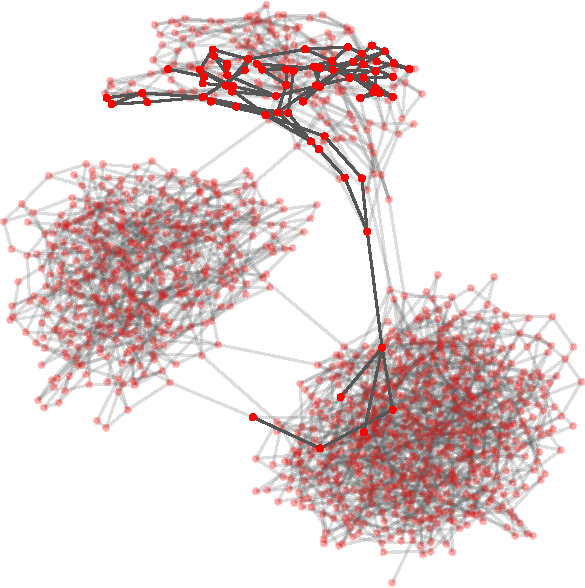
\includegraphics[width=0.25\textwidth]{batchRun__kHalf=2-2-2_maxUpdate=0.02_noize=0_nbrDepth=1/network750-crop.pdf}
\hfill
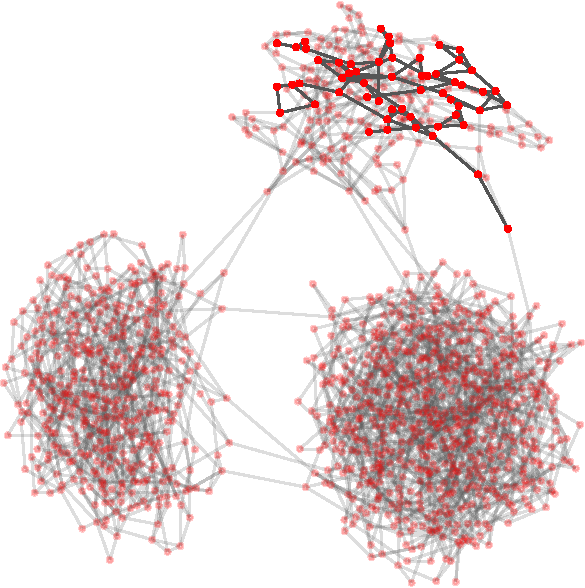
\includegraphics[width=0.25\textwidth]{batchRun__kHalf=2-2-2_maxUpdate=0.02_noize=0.01_nbrDepth=1/network750-crop.pdf}
\hfill
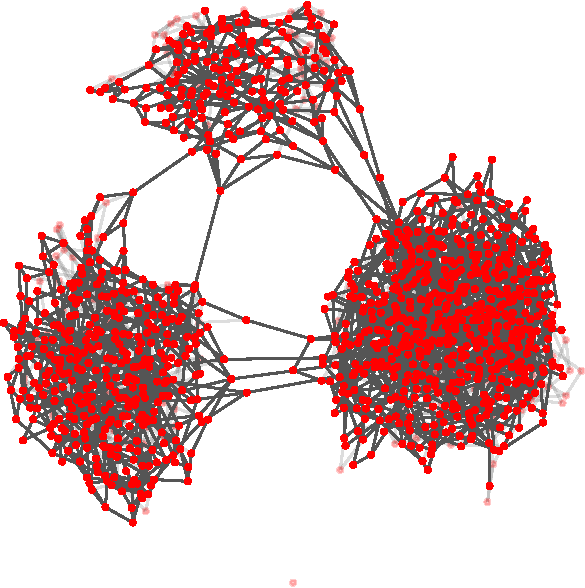
\includegraphics[width=0.25\textwidth]{batchRun__kHalf=2-2-2_maxUpdate=0.02_noize=0.1_nbrDepth=1/network750-crop.pdf}

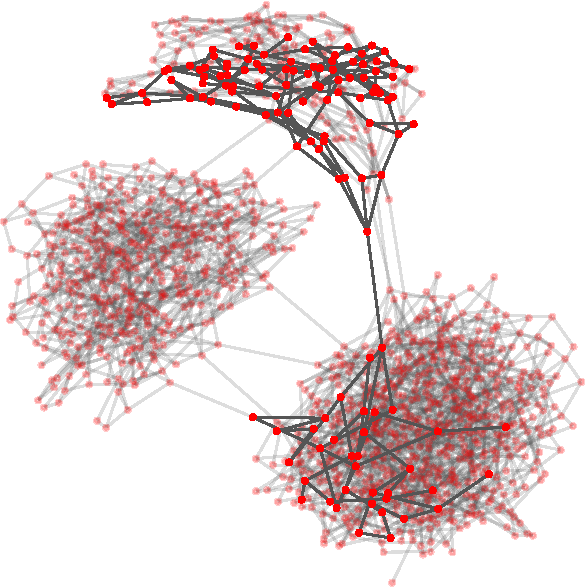
\includegraphics[width=0.25\textwidth]{batchRun__kHalf=2-2-2_maxUpdate=0.02_noize=0_nbrDepth=1/network1000-crop.pdf}
\hfill
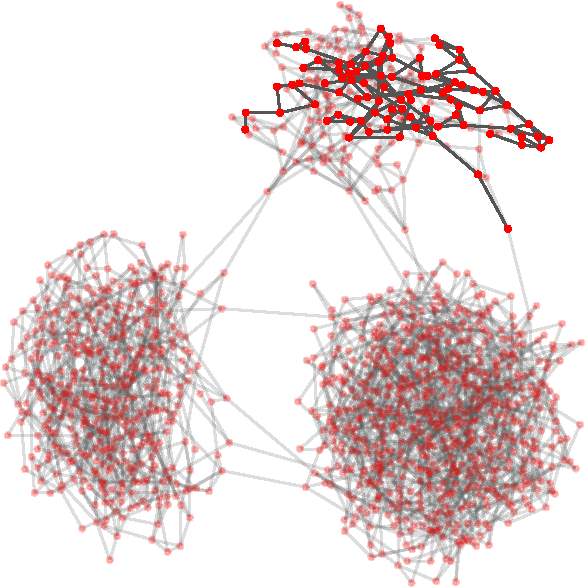
\includegraphics[width=0.25\textwidth]{batchRun__kHalf=2-2-2_maxUpdate=0.02_noize=0.01_nbrDepth=1/network1000-crop.pdf}
\hfill
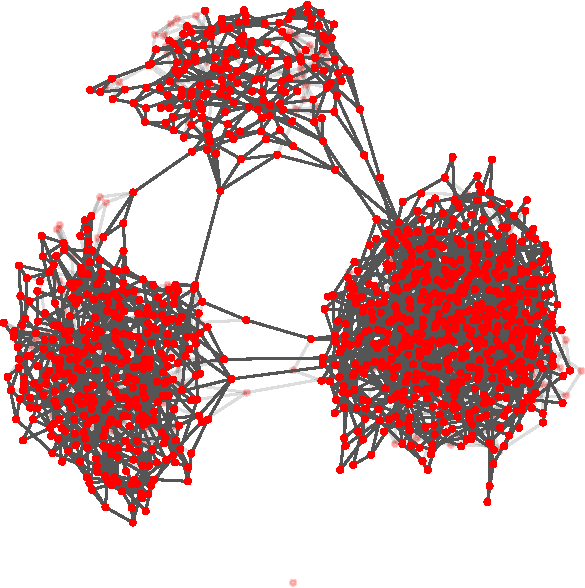
\includegraphics[width=0.25\textwidth]{batchRun__kHalf=2-2-2_maxUpdate=0.02_noize=0.1_nbrDepth=1/network1000-crop.pdf}

\caption{The influence of the noize for the three cases with on the left noize = 0, in the middle 0.01 and on the right 0.1. From top to bottom are the different time steps with the beginning and then increasing in 250 time steps till a 100 time steps.}
\label{influencenoize}
\end{figure}

\subsubsection{Influence of \texttt{maxAgentupdate}}
\label{sec:maxAgentUpdate}



\subsubsection{Influence of \texttt{nbrDepth} = Neighbor Depth}
\label{sec:nbrDepth}

\subsection{Influence of the network type}
\label{sec:influencenetworktype}

\subsection{Comparison to reality}
\label{sec:comparisontoreal}